\subsection{Scheduling Algorithms}\label{schedule algorithm}


\textbf{Notations}.
\begin{enumerate}
    \item \textbf{Assignment}: one feasible assignment (i.e. assign one task to one slot)
    \item $m=\sum \left |  \mathcal{T}_{k} \right |$ denote the amount of all dependent-free tasks.
\end{enumerate}

\subsubsection{Greedy Approach}\label{Greedy Approach}
~

Greedy Approach stems from a very natural intuition that we can schedule tasks to the idle slots with the shortest data transferring time, so that the sum completion time of each job in this small ``stage'' is also relatively short. 


    

\textbf{Procedure}. Compute a feasible assignment with shortest time. Bring this assignment into effect and repeat until all slots are full or all tasks have been assigned.

\textbf{Time Complexity}. We use priority queue to compute assignment with shortest time in $O(\log (|J|m))$. Thus, the time complexity is $O(m\log (|J|m))$. 

However, the greedy approach does not take max-min fairness into consideration. That is to say, it may improve the performances of some tasks while worsen others to achieve a relatively short sum completion time, which contradicts a lot with max-min fairness.
\subsubsection{K-Greedy Approach}\label{k-Greedy Approach}
~

\begin{figure}[htb]
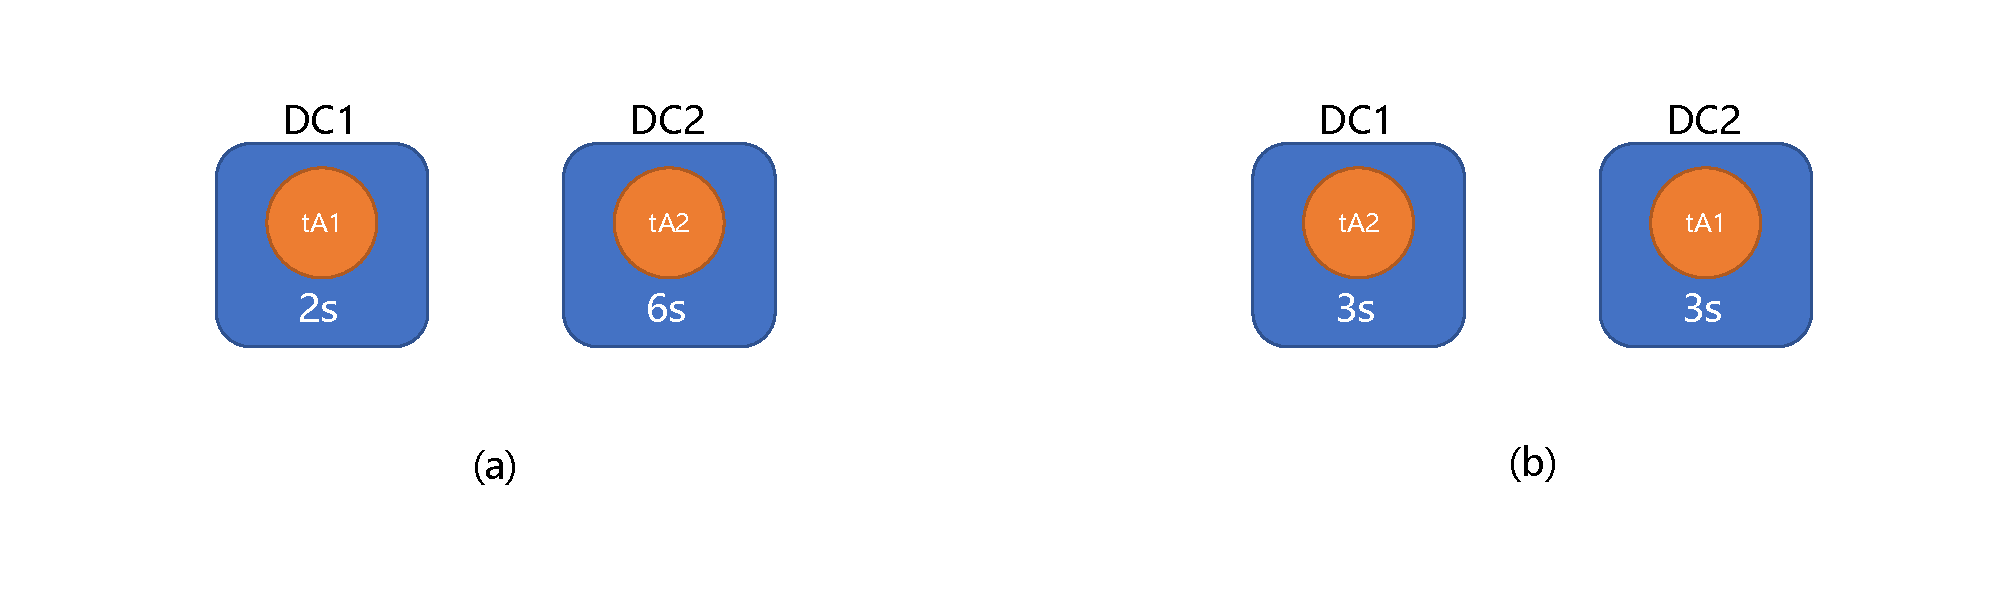
\includegraphics[width=1\textwidth]{figure/fig-greedy_eg.pdf}
\centering
\caption{Two possible assignments of tasks} \label{greedy_eg}
\end{figure}

When invoking Greedy Approach, we only consider about the very first task. And this may worsen the data transferring time of other tasks. This is better illustrated with example Fig. \ref{greedy_eg}. Greedy Approach first considers tA1 then tA2 and results in case (a). However, it is obvious that case (b) is better in both sum completion time and maximal completion time. Here, we introduce a randomized greedy approach, which is called K-Greedy Approach.

\textbf{Procedure}.
K-Greedy Approach randomly generate $k\sim U(0,2)$ for every task. Every time we compute an assignment with shortest data transferring time, we check whether $k$ is 0. If $k>0$, we simply skip this assignment and decrease $k$ by 1.

        % \begin{minipage}[t]{0.8\textwidth}
        %       \begin{algorithm}[H]
        %           %\LinesNumbered
        %           \KwIn{$x$, $y$}
        %           \KwOut{$sign$}
        %           \BlankLine
        %           \caption{$K-Greedy$} \label{Greedy_algo}

        %           $computes\ all\ possible\ assignments\ and\ put\ into\ priority\ queue$\;
        %           $randomly\ generate \ array\ K$\;
        %           $cnt \leftarrow 0$\;
        %           \While{$cnt < task\  number$}
        %           {
        %               $find\ assignment\ with\ shortest\ transferring\ time$\;
        %               $task \leftarrow assignment.task$\;
        %               \If{$K[task]>0 $ }
        %               {
        %                   $K[task]\leftarrow K[task]-1$\;
        %               }
        %               \ElseIf{$task \ is\ not\ assigned$}
        %               {
        %                   $bring\ this\ assignment\ into\ effect$\;
        %                   $cnt\leftarrow cnt+1$\;
        %               }
        %           }
        %       \end{algorithm}
        %   \end{minipage}

\textbf{Time Complexity}.
It may need k more iterations. Thus, time complexity is $O(km\log (|J|m))$.

K-Greedy Approach is able to yield case (b) in Fig. \ref{greedy_eg}. However, as $k$ is randomly generated, its performance is not so stable. Worse still, it may make unnecessary concessions and worsen the performance. 


\subsubsection{Network-Flow-Based Greedy Approach}\label{NFBGA}
~

K-Greedy Approach is able to yield better solution sometimes, but with poor stability. This raises a natural question, can we find an approach to minimize the sum data transferring time of $k$ tasks without randomness? The answer is YES and we can use a network-flow-based algorithm to achieve this, which computes maximal flow while maintain minimal cost sum.

\textbf{Construction}. 
    We construct a weighted network graph $G=(V,E,s,t,c_e,w_e)$, where $c_e$ is the capacity of edge and $w_e$ is the cost of edge. When there is $f(e)$ flow in $e$, we will add $f(e) \cdot w_e$ to total cost.
    
\begin{enumerate}
    \item
        To begin with, $s$ is virtual source and it connects DC $i$ with $c_e=a_i$ and $w_e=0$. This ensures we can not assign more tasks into one DC than the amount of its idle slots.
    \item
        For each DC $i$, it has exactly $m$ edges.
        Each edge connects to one task, say task $i$ of job $k$, with $c_e=1$ and $w_e=c_{i,j}^k$.
        $c_e=1$ ensures each task can only be assigned once while $w_e$ indicates the cost of this assignment.
        This results in  $\left | J \right | \cdot m $ edges in total, which cover all possible assignments.
        Here, we denote these edges as \textbf{Assignment Edges}.
        
    \item
        Finally, $t$ is a virtual sink and every task connects to it with $c_e=1$ and $w_e$.
\end{enumerate}
    In Fig. \ref{fig-network_greedy}, (a) shows the network we construct and (b) shows the maximal flow with minimal cost of this network.
  
\begin{figure}[htb]
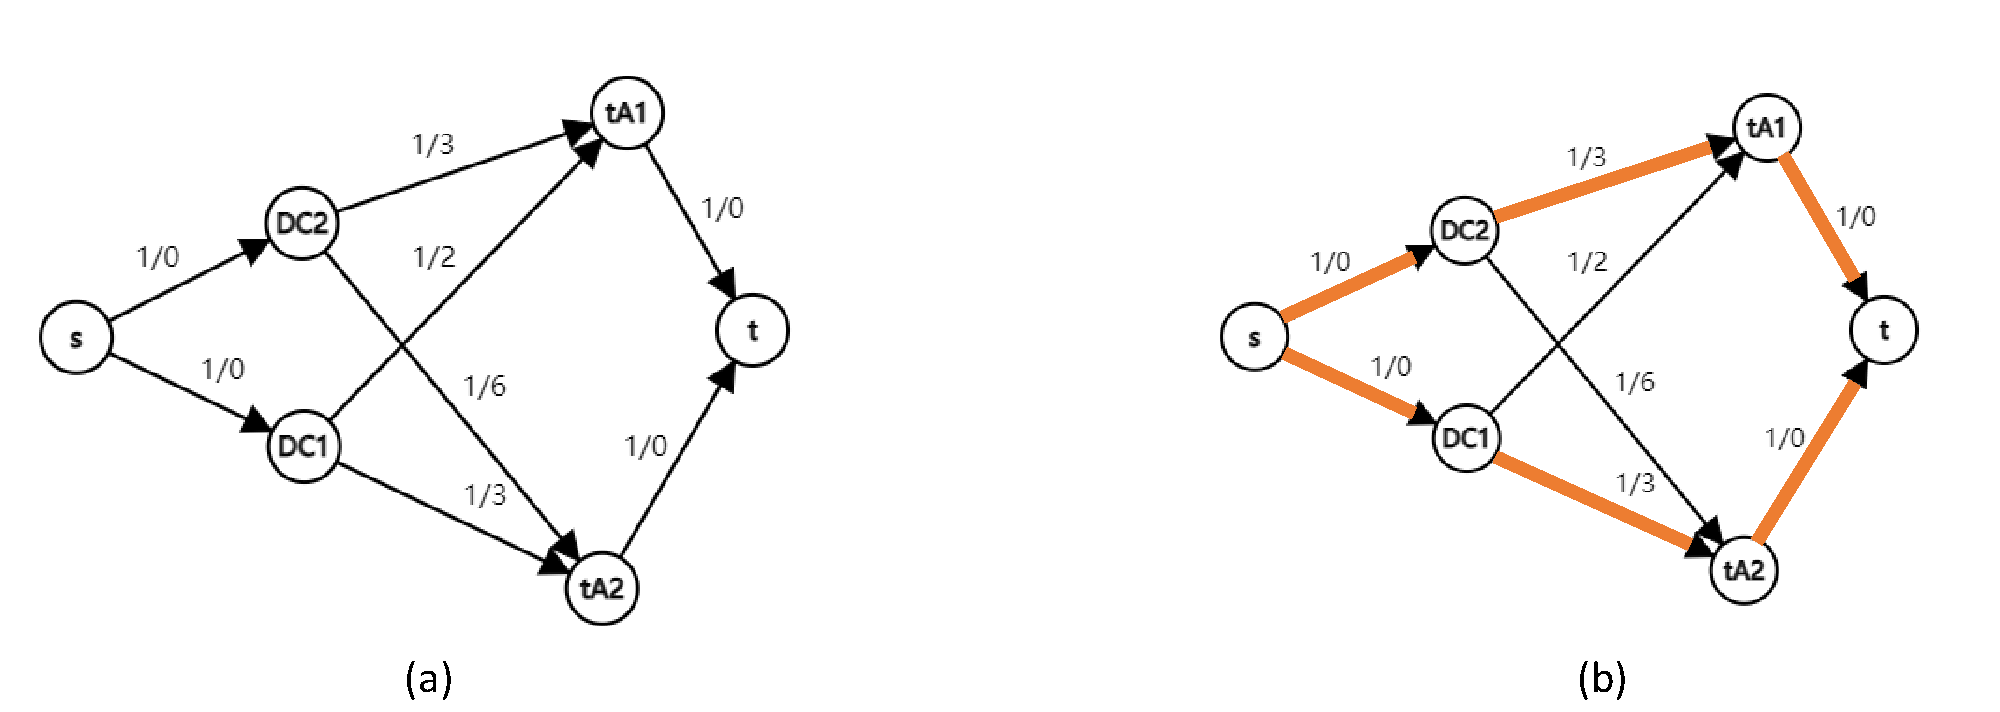
\includegraphics[width=1\textwidth]{figure/fig-network_greedy.pdf}
\centering
\caption{(a) network of Fig. \ref{greedy_eg}.  Each edges have capacity / weight. (b) maximal flow with minimal cost} \label{fig-network_greedy}
\end{figure}  

\textbf{Solve}. To solves maximal flow with minimal cost, we can apply Bellman-Ford Algorithm to find shortest (i.e. minimal cost sum) augmenting path each iteration. As the cost is minimized, we minimize the sum data transferring time of tasks counted in maximal flow. To get the final assignments, we check each \textbf{Assignment Edge}. If $f(e)=1$, then it indicates this assignment is chosen in maximal flow and we bring this assignment into effect.

\textbf{Time Complexity}. The network has $O(|J|+m)$ nodes and $O(\left | J \right | m)$ edges. Thus, the time complexity is $O(|J|^2m+|J|m^2) $.


\textbf{Example}. This is better illustrate with example in Fig. \ref{greedy_eg}. And Fig. \ref{fig-network_greedy} is the corresponding network graph we construct. If we apply Greedy Approach, it will first assign tA1 to DC1 and tA2 to DC2, which yields case (a) and a total data transferring time of $2+6=8$. However, if apply network-flow-based Greedy Approach to consider these two tasks simultaneously, we are able to get case (b) and a total data transferring time $3+3=6$.


\subsubsection{Network-Flow-Based Fair Approach}\label{NFBFA}
~

Network-Flow-Base Greedy Approach only ensures that the sum data transferring time of $k$ tasks is minimized. However, it does not achieve max-min fairness and may suffer from same problem as Greedy Approach. Here, we introduce a Network-Flow-Based Fair Approach, which can achieve max-min fairness.

\textbf{Construction}. We construct the network graph similar to Network-Flow-Based Greedy Approach. But take both data transferring time and execute time into consideration (i.e. $w_e=c^k_{i,j}+e^k_{i,j}$).  

\textbf{Solve}. To achieve max-min fairness, we need first to minimize $\max\{c^k_{i,j}+e^k_{i,j}\}$. It is quite hard to find the optimal solution. However, to certificate it is much easier.  

Let $\Delta$ denote the answer.
\begin{enumerate}
    \item \textbf{Certifier}. Given a $\Delta$, let $G(\Delta)$ be the subgraph of $G$ consisting of only edges with $w_e\leq \Delta$. Then, we compute maximal flow in $G(\Delta)$. If $f_{max}=m$, then it indicates we can assign all dependent-free tasks within bottleneck $\Delta$.
    
    \item \textbf{Search $\Delta$}. Since, we already have a certifier. The remaining work is to find $\Delta$. We can observe that $\Delta$ is monotonic. In other words, given $\Delta_{min}$, $\Delta \geq \Delta_{min}$ are feasible solutions while $\Delta < \Delta_{min} $ are not. Thus, we can use binary search to accelerate the search of $\Delta$.
    
    \item \textbf{Max-Min Fairness}. Once we find the bottleneck of some tasks, the corresponding job's finish time can be better. Thus, we can assign other tasks (denoted by $ \mathcal{T}^{'}_{k}$) in the same job more arbitrarily as long as they do not worsen bottleneck. To achieve this, for each task in $ \mathcal{T}^{'}_{k}$, we check every corresponding edge in network graph. 
    \begin{enumerate}
        \item  If $w_e> bottleneck$, we can not bring this assignment into effect or it would worsen bottleneck. Thus, we need to set $w_e^{'}=\infty$ to ensure this edge will not be chose. 
        \item  If $w_e\leq bottleneck$, we just do the opposite and set $w_e^{'}=0$. This ensures these assignments will not affect finding bottleneck of other jobs.
    \end{enumerate}
    Moreover, we bring bottleneck assignment into effect and decrease DC capacity accordingly.
    After updating the network graph, we repeat the procedure and find the bottleneck of next job. Finally this procedure finishes when we find bottleneck of each job.
    
\end{enumerate} 
    
\begin{figure}[htb]
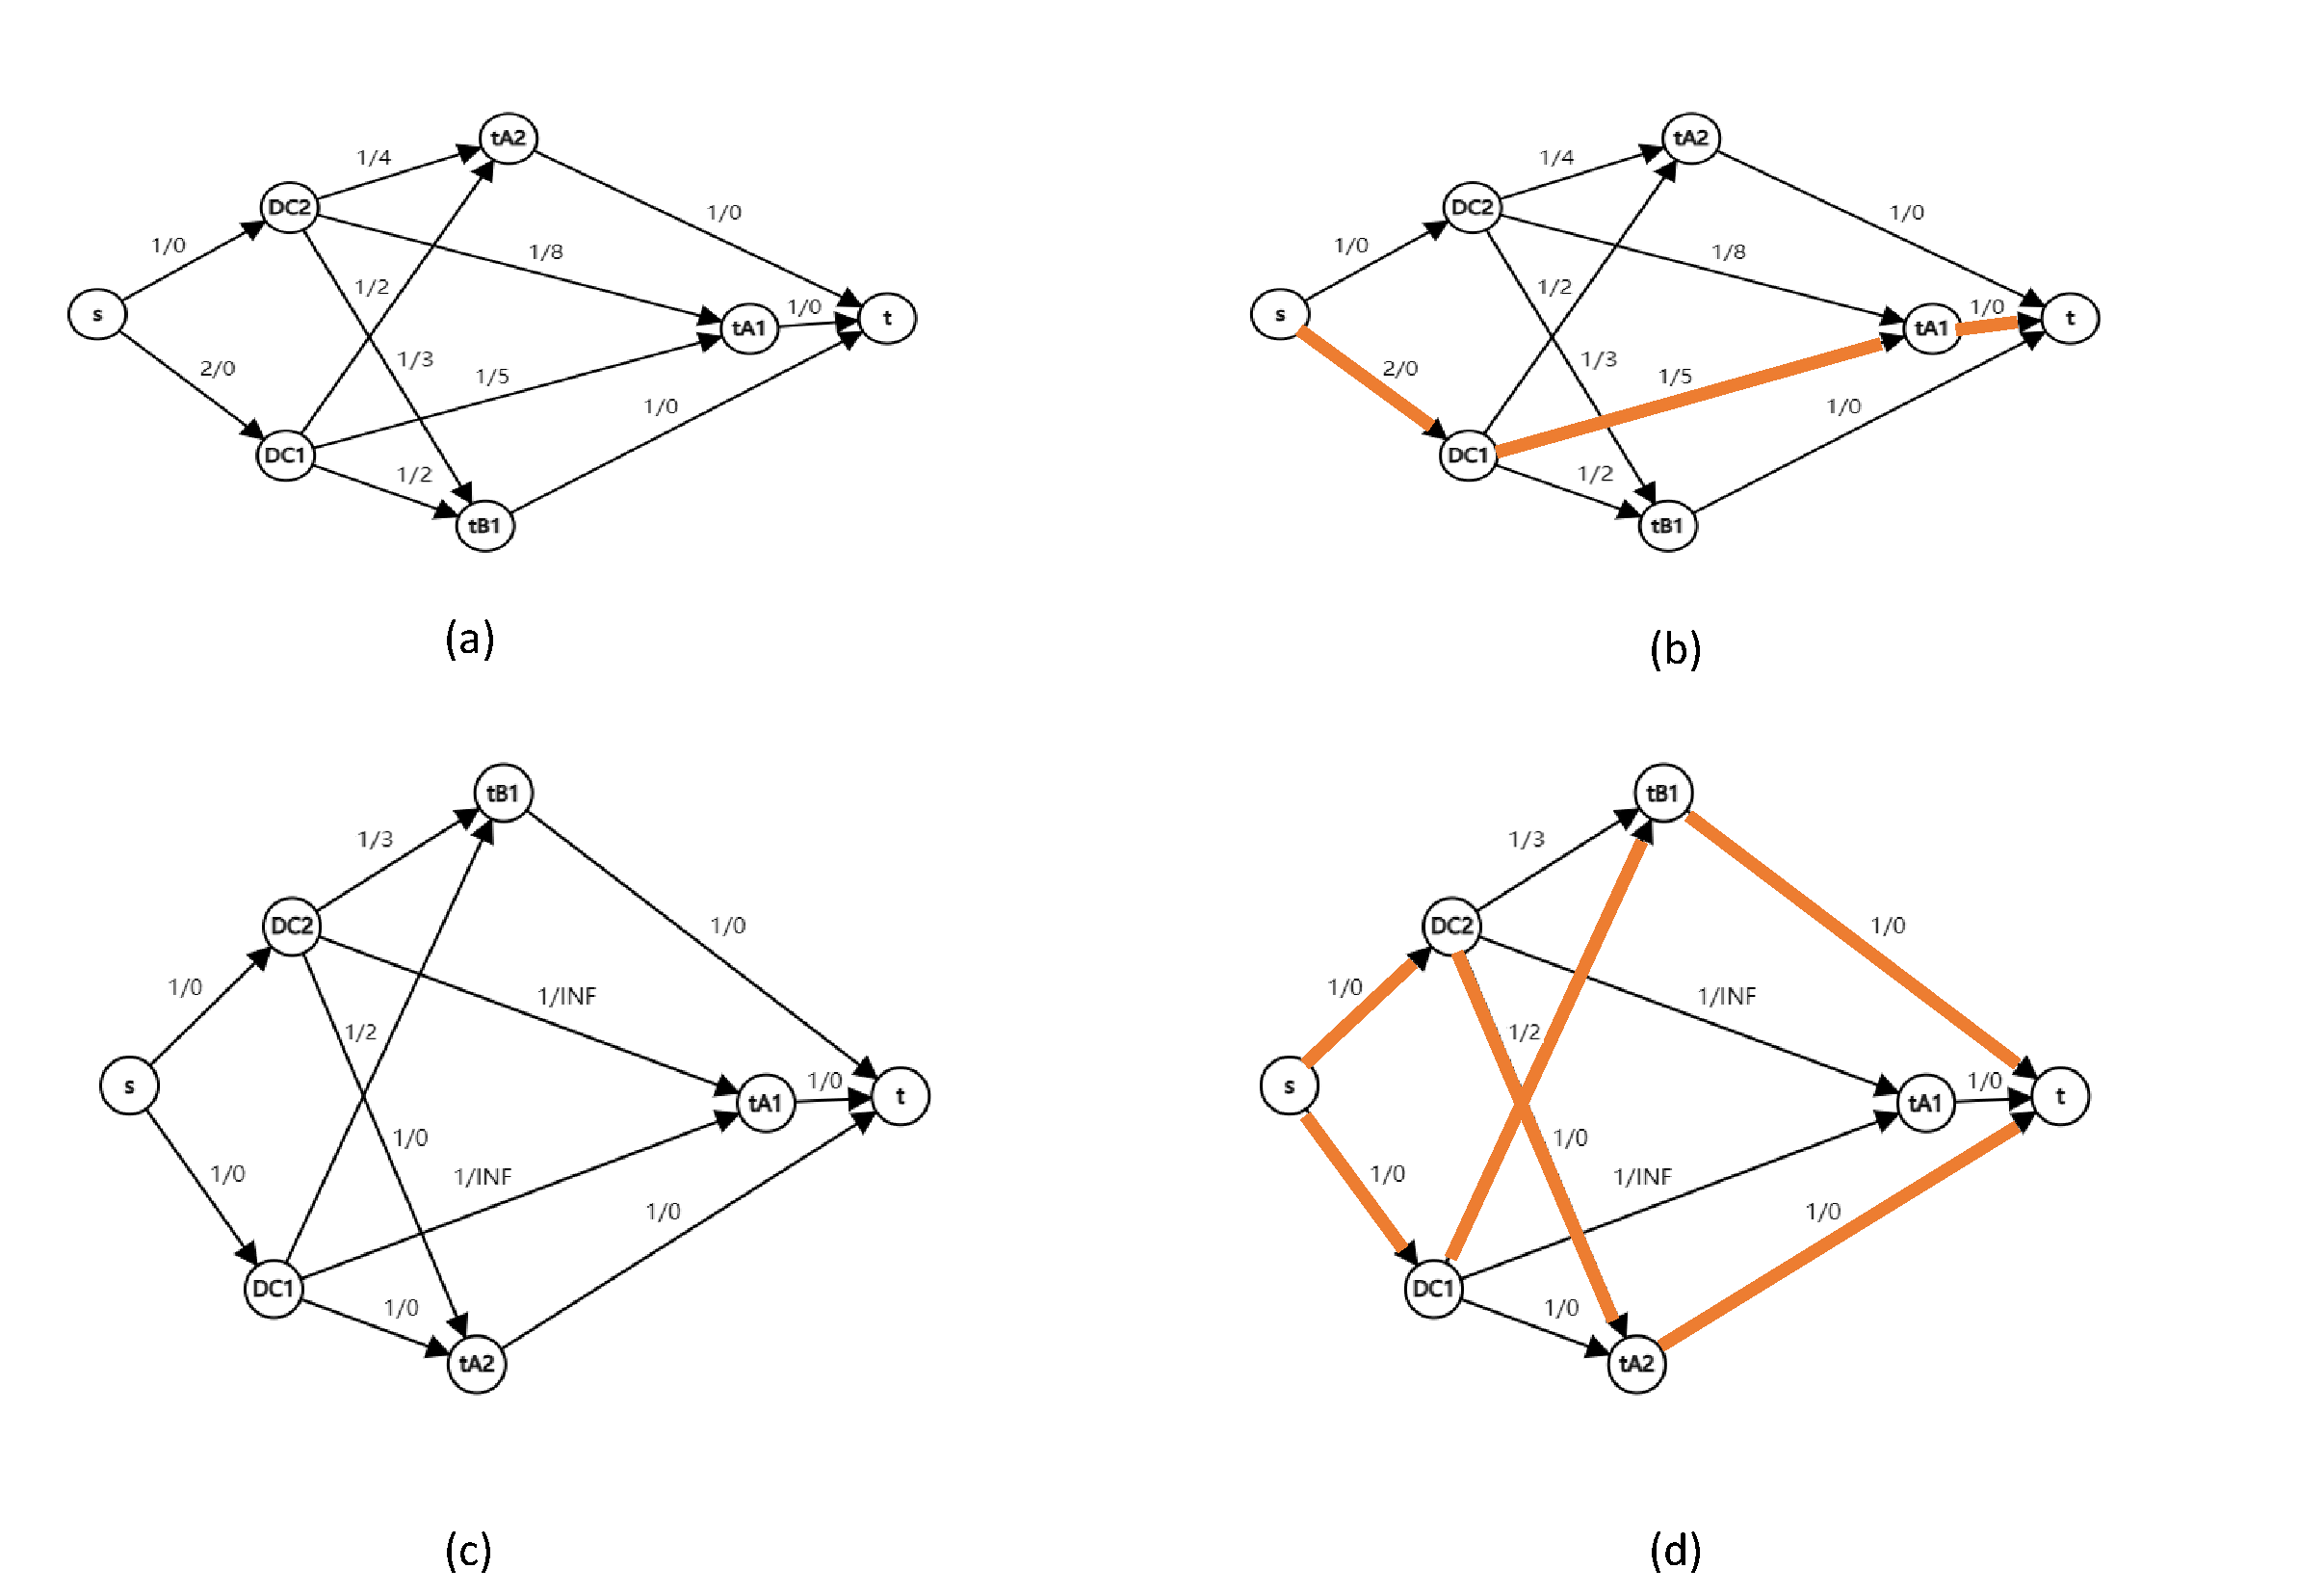
\includegraphics[width=1\textwidth]{figure/fig-fair.pdf}
\centering
\caption{Max-min fairness example.} \label{fig-fair}
\end{figure}
    
\textbf{Time Complexity}.Certifier takes $O(|J|^2m+|J|m^2)$ and binary search takes $O(\log(\max\{c_e\}) )$. Beside, we need $|\mathcal{K}|$ iterations to find bottleneck in each job respectively. Thus, the time complexity of Network-Flow-Based Fair Approach is $O((|J|^2m+|J|m^2)\log (\max \{c_e\}) |\mathcal{K}|)$.

\textbf{Example}. To illustrate better how Network-Flow-Based Fair Approach achieve max-min fairness, we introduce a new example Fig. \ref{fig-fair}. Suppose after construct we have network graph (a). We apply Network-Flow-Based Fair Approach on this and (b) shows the result of first iteration. After first iteration, we find assigning tA1 to DC1 is the bottleneck with $w_e=5$. Thus, we assign tA1 to DC1 and update the network graph accordingly. (c) shows the new network graph, where edges of job A are either $0$ or $\infty$. We repeat the procedure again and this time we find assigning tB1 to DC1 is the bottleneck with $w_e=2$. As there are only 2 jobs and we find 2 bottlenecks, the algorithm terminates with max-min fairness solution (tA1,tA2,tB1)$=(5,4,2)$.
Note that Greedy Base Approach can never give this solution as $(5,2,3)$ minimize the sum completion time.
    
